% finite-cylinder.tex

\section{Flow of nitrogen over a cylinder of finite length}
\label{sec:finite-cyl-sec}
%
This example is relevant to Troy and Tim's X2 experiments on flows of weakly-ionizing
nitrogen over cylinders of various length over diameter ratios.
It exercises the three-dimensional flow solver with a strong bluff-body shock and
a very sudden expansion over the end of the cylinder.
The thermochemical module is also exercised with both near-equilibrium and frozen thermochemistry
regions in the flow field and temperatures that rise above 20\,000\,K.
Two simulations of the cylinder flow are presented: the first with chemical nonequilibrium and thermal equilibrium, and 
the second with both chemical and thermal nonequilibrium.

\medskip
The flow domain shown is made up of 4 block-structured grids as shown in Figure\,\ref{finite-cyl-layout}
and number of the surface grids are are indicated in Figure\,\ref{finite-cyl-p-fig} for a 15\,mm diameter cylinder 
with $\frac{L}{D} = 2$.
Note that only half of the length and only the upper-front quarter 
of the cylinder is in the simulation.
Slip-wall boundary conditions are used (implicitly) along the planes of symmetry.

\begin{figure}[htbp]
\hbox{
  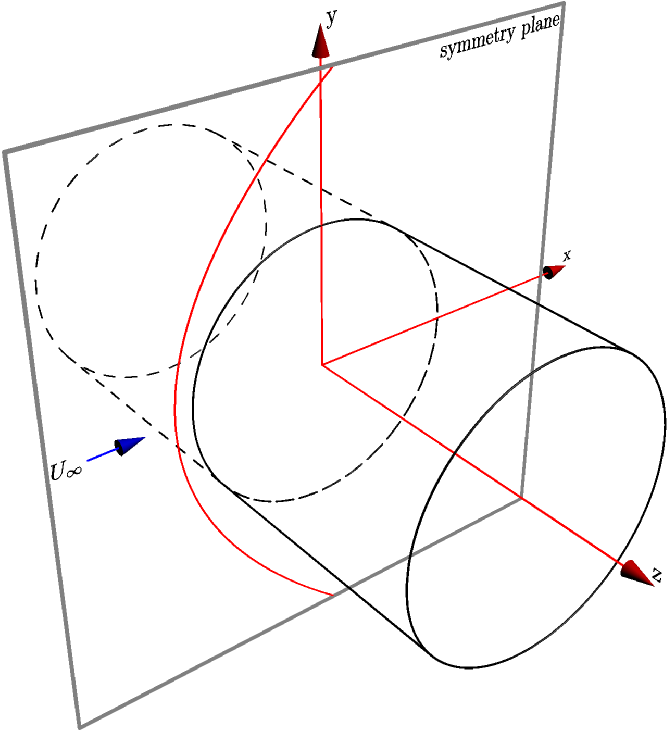
\includegraphics[width=0.5\textwidth]{../3D/finite-cylinder/schematics/full-cyl-schematic.pdf}
  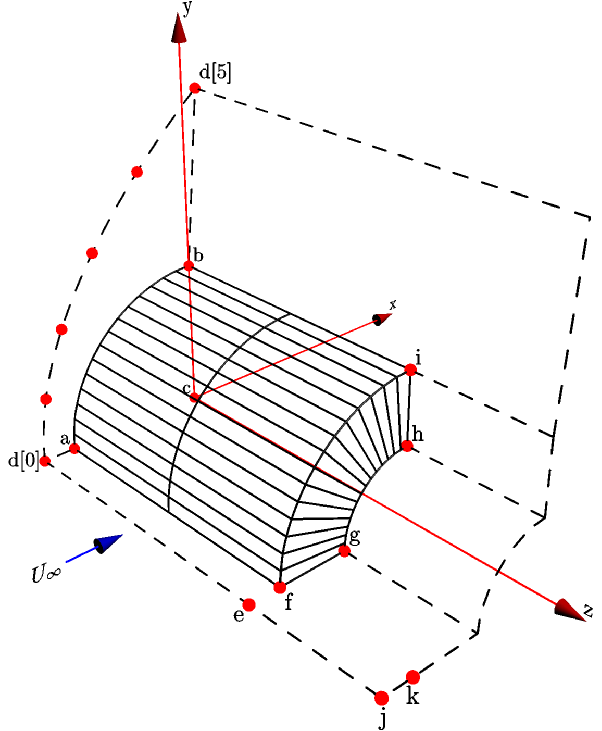
\includegraphics[width=0.5\textwidth]{../3D/finite-cylinder/schematics/cyl-schematic.pdf}
}
\caption{Left: full cylinder with the expected shock location scribed on the symmetry plane.
   Right: layout of finite-cylinder simulation with one-quarter of forward-facing half 
   of the cylinder surface shown as wire-frame.
   Some of the edges of the flow domain are shown dashed and
   the labelled nodes correspond to those in the input script.}
\label{finite-cyl-layout}
\end{figure}

\medskip 
The free-stream conditions ($p_{\infty} = 2$\,kPa, $T_{\infty} = 3000$\,K
and $u_{\infty} = 10$\,km/s) correspond approximately to Troy's X2 experiments.
These are representative of those produced by the X2 expansion tube and,
for an ideal nitrogen test gas, the free stream Mach number is 8.96.

\subsection{Chemical nonequilibrium and thermal equilibrium}

\medskip
Here we describe the finite-cylinder simulations with chemical nonequilibrium and thermal equilibrium.
This means chemical reactions are permitted to occur at a finite-rate (chemical nonequilibrium), but all thermal modes 
are assumed to be governed by a single temperature (thermal equilibrium).

\medskip
The script sets up the simulation to run for 30 flow-lengths ($30 * R_c / u_{\infty}$)
and the final time reached is 22.5\,$\mu$s
The relieving effect on the shock is clear in both the pressure and temperature field (Figure\,\ref{finite-cyl-T-fig}).
The temperature field also shows the influence of the finite-rate reactions with peak temperatures immediately
behind the shock, followed by a relaxation as dissociation of the nitrogen molecules soaks up energy from within the 
shock layer.
 
\begin{figure}[htbp]
\begin{center}
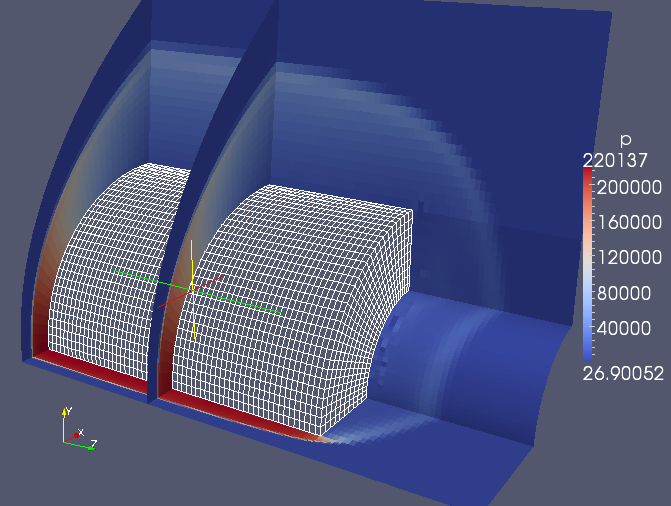
\includegraphics[width=9.5cm]{../3D/finite-cylinder/thermal-eq/finite-cyl-p-with-mesh-aug2010.png}
\end{center}
\caption{A selection of surface grids from the finite-cylinder simulation with chemical nonequilibrium, 
   shown as wire-frame on the cylinder surface
   and coloured by pressure in the flow field.
   This PNG figure was generated with Paraview using block surfaces extrtacted from final solution file.}
\label{finite-cyl-p-fig}
\end{figure}

\medskip
This case is quite difficult for both the flow solver and the finite-rate chemistry module
and defects can be seen in the solution around the flat end of the cylinder and toward the
outflow boundaries.
These defects are quite obvious in the temperature field with a checker-board pattern of
extreme high and low temperatures.
However, the forebody flow looks to be reliably computed and the shock stand-off distance is
1.13\,mm near the midplane of the cylinder.

\begin{figure}[htbp]
\hbox{
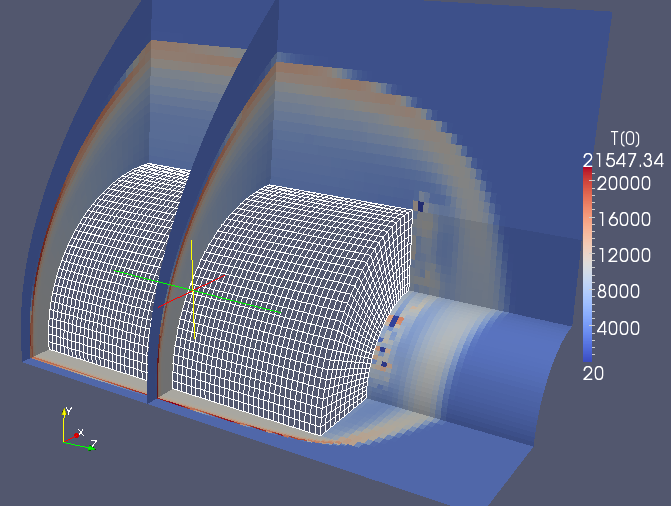
\includegraphics[width=0.5\textwidth]{../3D/finite-cylinder/thermal-eq/finite-cyl-T-with-mesh-aug2010.png}
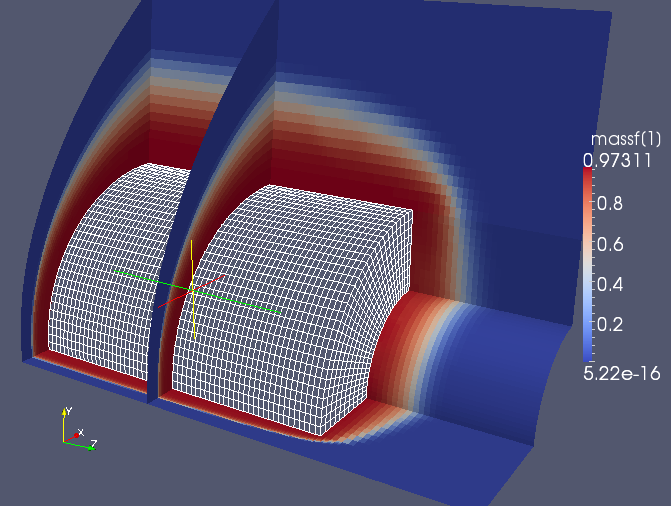
\includegraphics[width=0.5\textwidth]{../3D/finite-cylinder/thermal-eq/finite-cyl-N-massf-with-mesh-aug2010.png}
}
\caption{Static temperature and mass fraction of nitrogen atoms in the flow field from the chemical nonequilibrium simulation.}
\label{finite-cyl-T-fig}
\end{figure}



\clearpage

\subsubsection{Input script (.py)}\index{block!SuperBlock3D!example of use}\index{chemical reaction!example of use}
\label{finite-cyl-script}
\topbar
\lstinputlisting[language={}]{../3D/finite-cylinder/thermal-eq/cyl.py}
\bottombar

\subsubsection{Reaction scheme file (.lua)}\index{chemical reaction!reaction scheme file!weakly-ionising nitrogen}
\topbar
\lstinputlisting[language={}]{../3D/finite-cylinder/thermal-eq/nitrogen-5sp-6r.lua}
\bottombar

\pagebreak
\subsubsection{Shell script}\index{e3mpi.exe!example of use}
\label{finite-cyl-sh-files}
\topbar
\lstinputlisting[language={}]{../3D/finite-cylinder/thermal-eq/run_simulation.sh}
\bottombar


\subsubsection{Postprocessing program}\index{postprocessing!customized!shock location}
\label{finite-cyl-post-files}
\topbar
\lstinputlisting[language={}]{../3D/finite-cylinder/thermal-eq/post_simulation.sh}
\bottombar\\
\topbar
\lstinputlisting[language={}]{../3D/finite-cylinder/thermal-eq/locate_bow_shock.py}
\bottombar

\subsubsection{Notes}
\begin{itemize}
\item It is well worth the bother to run this simulation on multiple processors. 
  The elapsed time for the run with 4 MPI processes is 9193\,seconds on geyser,
  a Dell server with $4\times4$ AMD cores.
  Of course, our MPI job used only 4 of those cores.
\item We tried a couple of reconstruction variations.  
  The original simulation required 5999 steps using \texttt{rhoe} interpolation.
  Using \texttt{pT} interpolation (as shown in the script), the simulation required 
  an elapsed computing time of 8492\,seconds and 6025 steps on \texttt{geyser} in January 2010.
  In August 2010, the same calculation took 4315\,seconds on 4 cores of the barrine cluster 
  to do 6023 steps at final time.
\item To double the grid resolution (as one might want to do for a convergence
  study), would require a factor of 8 increase in memory.
  If you are planning to do calculations of any reasonable complexity, it is
  worth your while to invest in learning to use the cluster computer and
  the parallel version of the code.
\end{itemize}

\subsection{Chemical and thermal nonequilibrium}
\label{finite-cyl-therm-noneq}

\medskip
Here we describe the finite-cylinder simulations with both chemical and thermal nonequilibrium.
Specifically, a two-temperature thermal model as proposed by Park~\cite{park_1989} is implemented.
This means chemical reactions are permitted to occur at a finite-rate (chemical nonequilibrium), and the translation and rotation thermal modes are governed by one temperature $T_\text{tr}$ and the vibration and electronic thermal modes by a separate temperature $T_\text{ve}$ 

\begin{figure}[htbp]
\subfloat[Translation-rotation temperature, p]{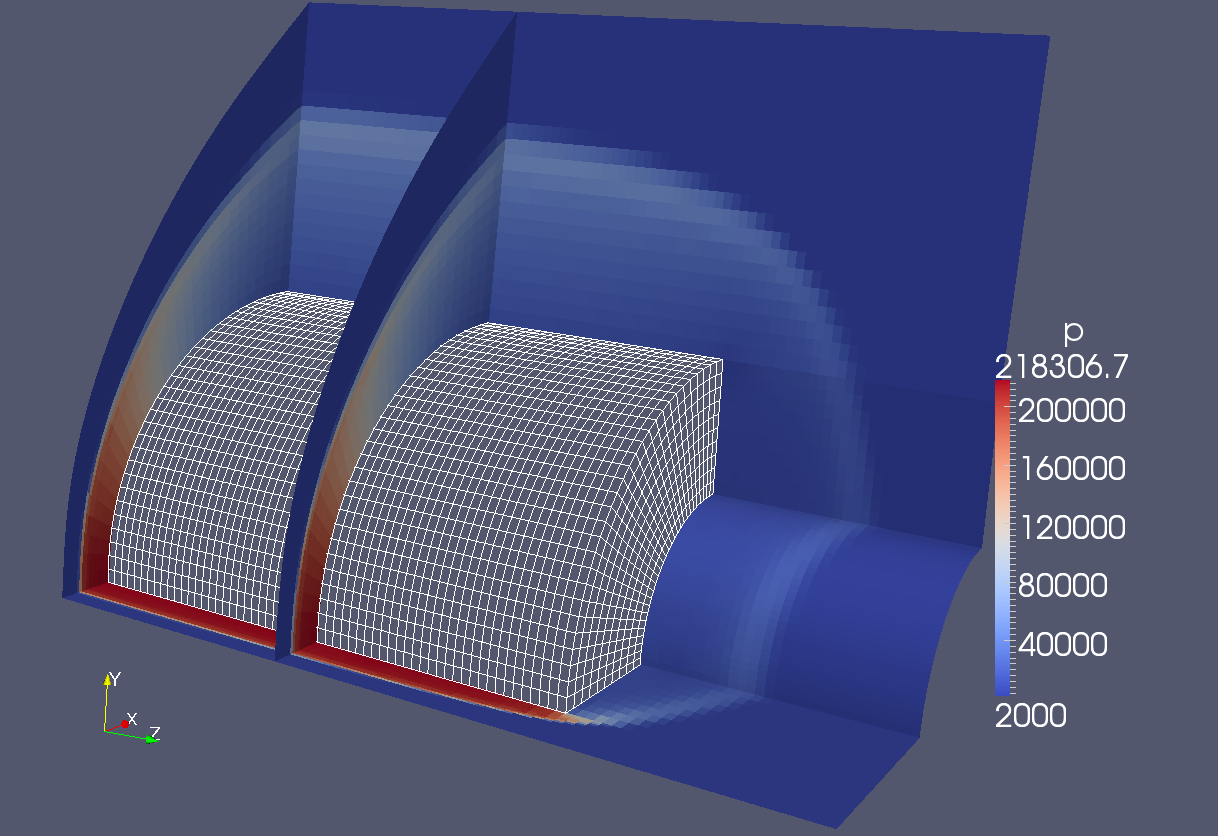
\includegraphics[width=0.5\textwidth]{../3D/finite-cylinder/thermal-noneq/finite-cyl-p-with-mesh-dec2011.png}} \hspace{1mm}
\subfloat[Atomic nitrogen mass-fraction, $f_\text{N$_2$}$]{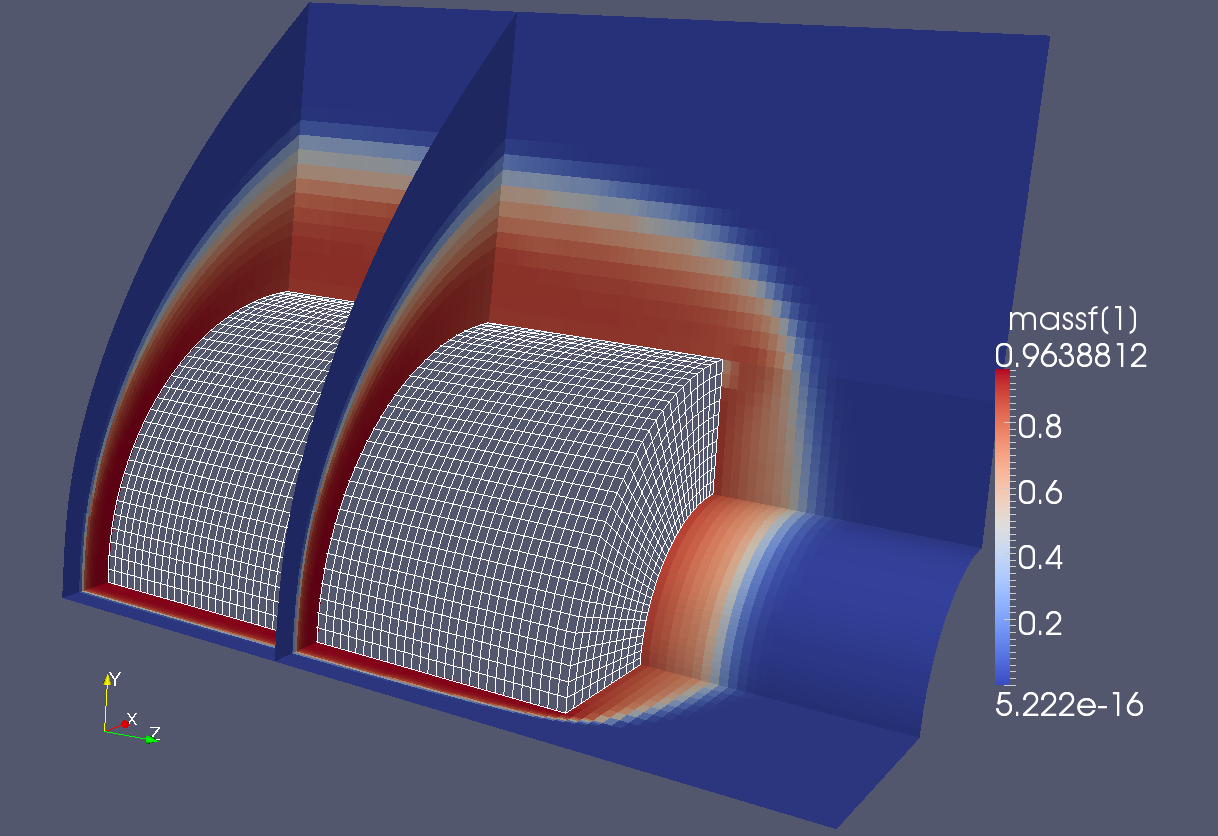
\includegraphics[width=0.5\textwidth]{../3D/finite-cylinder/thermal-noneq/finite-cyl-N-massf-with-mesh-dec2011.png}} \\
\subfloat[Translation-rotation temperature, $T_\text{tr}$]{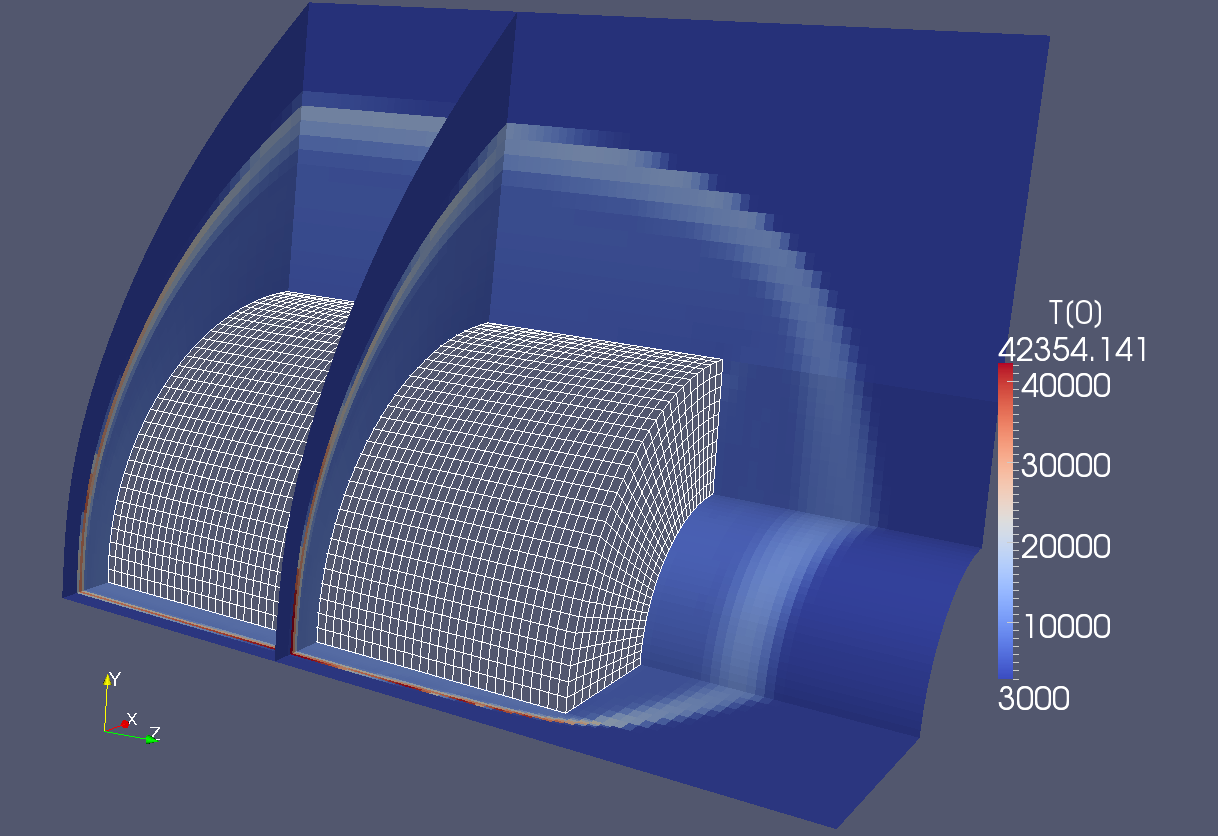
\includegraphics[width=0.5\textwidth]{../3D/finite-cylinder/thermal-noneq/finite-cyl-Ttr-with-mesh-dec2011.png}} \hspace{1mm}
\subfloat[Vibration-electron-electronic temperature, $T_\text{ve}$]{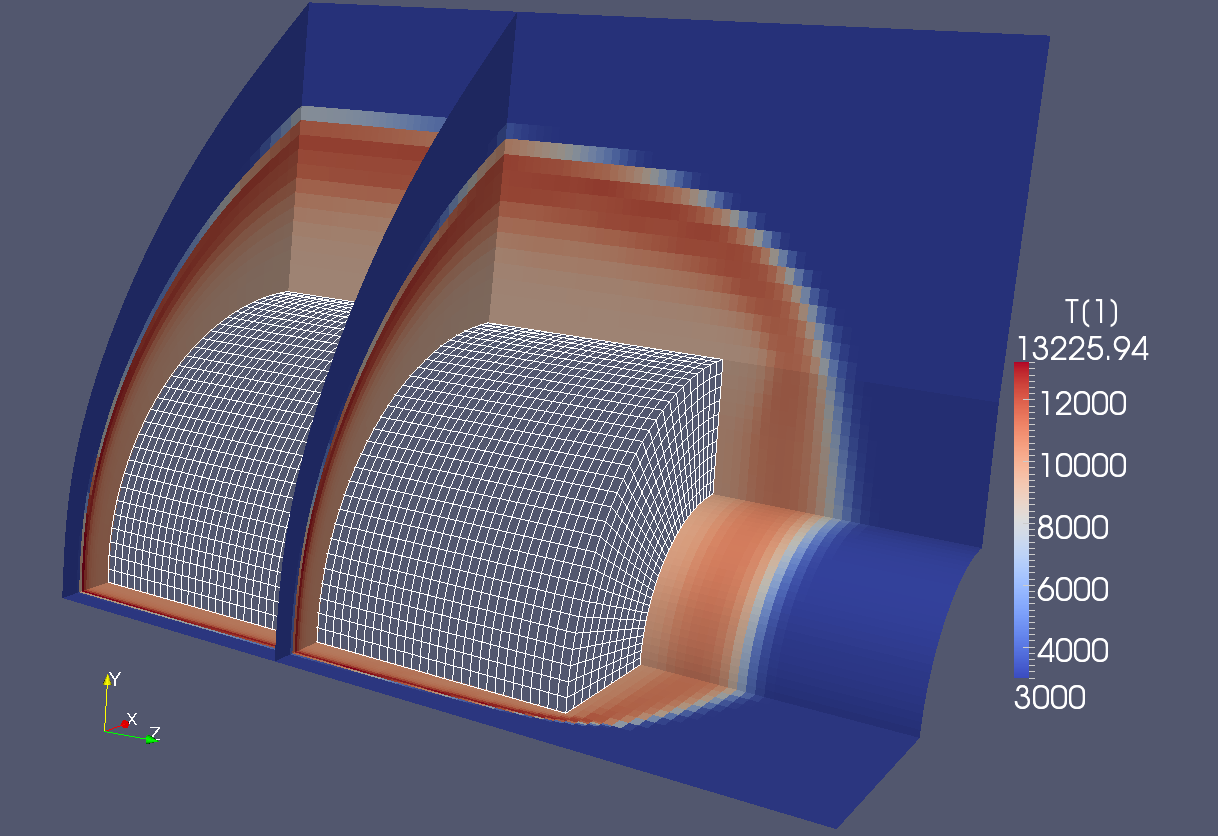
\includegraphics[width=0.5\textwidth]{../3D/finite-cylinder/thermal-noneq/finite-cyl-Tve-with-mesh-dec2011.png}}
\caption{Flow field contour plots from the thermal nonequilibrium simulation.}
\label{finite-cyl-TNE-contours}
\end{figure}

\begin{figure}[htbp]
\subfloat[Temperature profile]{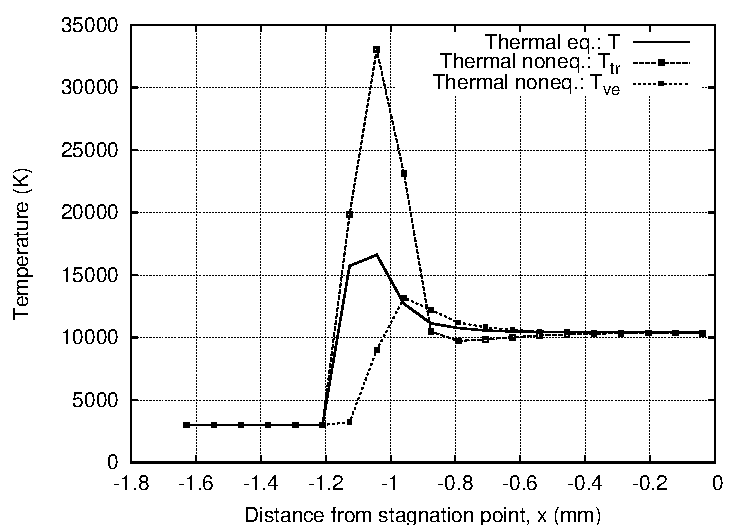
\includegraphics[width=0.5\textwidth]{../3D/finite-cylinder/thermal-noneq/temperature_profiles.pdf}}
\subfloat[Diatomic nitrogren density profile]{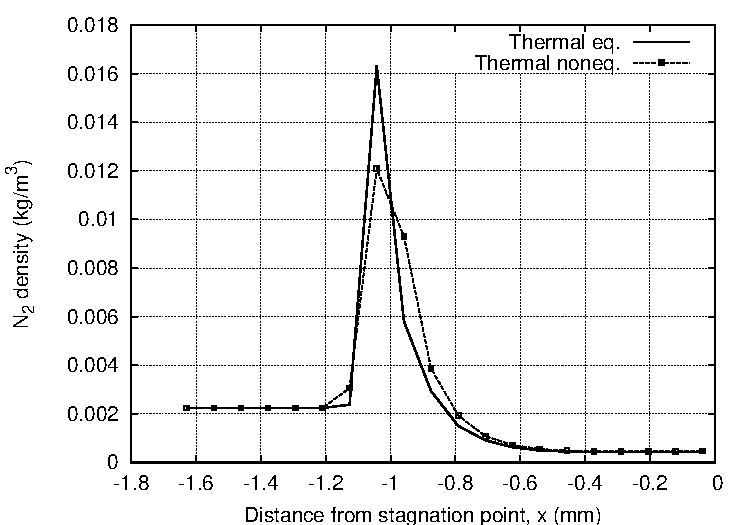
\includegraphics[width=0.5\textwidth]{../3D/finite-cylinder/thermal-noneq/N2_profiles.pdf}}
\caption{Stagnation-line profile plots from the thermal nonequilibrium simulation.}
\label{finite-cyl-TNE-profiles}
\end{figure}

\clearpage

\subsubsection{Input script (.py)}\index{block!SuperBlock3D!example of use}\index{thermal nonequilibrium!example of use}
\label{finite-cyl-script-2T}
\topbar
\lstinputlisting[language={}]{../3D/finite-cylinder/thermal-noneq/cyl.py}
\bottombar

\subsubsection{Reaction scheme file (.lua)}\index{chemical reaction!thermal nonequilibrium reaction scheme file!weakly-ionising nitrogen}
\topbar
\lstinputlisting[language={}]{../3D/finite-cylinder/thermal-noneq/nitrogen-5sp-6r.lua}
\bottombar

\subsubsection{Energy exchange scheme file (.lua)}\index{energy exchange!energy exchange scheme file!weakly-ionising nitrogen}
\topbar
\lstinputlisting[language={}]{../3D/finite-cylinder/thermal-noneq/TV-TE_exchange.lua}
\bottombar

\pagebreak
\subsubsection{Shell script}\index{e3mpi.exe!example of use}
\label{finite-cyl-sh-files-2T}
\topbar
\lstinputlisting[language={}]{../3D/finite-cylinder/thermal-noneq/run_simulation.sh}
\bottombar


\subsubsection{Postprocessing program}\index{postprocessing!customized!shock location}
\label{finite-cyl-post-files-2T}
\topbar
\lstinputlisting[language={}]{../3D/finite-cylinder/thermal-noneq/post_simulation.sh}
\bottombar\\
\topbar
\lstinputlisting[language={}]{../3D/finite-cylinder/thermal-noneq/locate_bow_shock.py}
\bottombar

\subsubsection{Notes}
\begin{itemize}
\item The elapsed time for this simulation was 12895\,seconds on 4 CPU's of the barrine cluster.
  On the same hardware the thermal equilibrium version of this simulation took 4130\,seconds --- 
  a three-fold increase in computation time.  This is to be expected as the implementation of a 
  thermal nonequilibrium model introduces an additional conserved quantity to be accounted for (vibration-electron-electronic energy), 
  and requires the ODE system for thermal energy exchange to be solved.
\end{itemize}

